\documentclass[11pt,letterpaper]{article}
\usepackage[top=1.00in, bottom=1.0in, left=1in, right=1in]{geometry}
\usepackage{textcomp}
\usepackage{amsfonts}
\usepackage{verbatim}
\usepackage[english]{babel}
\usepackage{pifont}
\usepackage{color}
\usepackage{setspace}
\usepackage{lscape}\parskip=5pt
\usepackage{gensymb} % You have to have this to use \degree
\usepackage{float}
\usepackage{latexsym}
\usepackage{url}

% Reference Supp labels
\usepackage{zref-xr}
\zxrsetup{toltxlabel=true, tozreflabel=false}
\zexternaldocument*{winefuture_supp}
\usepackage{epsfig}
\usepackage{graphicx}
\usepackage{amssymb}
\usepackage{amsmath}

\usepackage{caption}
\usepackage{lineno}
\usepackage[utf8]{inputenc}
\usepackage{sectsty,setspace,natbib}
\usepackage{graphicx}
\usepackage{latexsym,epsf,rotating}
\usepackage{epstopdf}

\linespread{1.2} % was 1.66 for double-spaced 
% \raggedright
\setlength{\parindent}{0.5in}

\setcounter{secnumdepth}{0}

\pagestyle{empty}

\renewcommand{\tableofcontents}{}

\parskip=5pt
\pagenumbering{arabic}
\pagestyle{plain}

\usepackage{fancyhdr}
\pagestyle{fancy}
\fancyhead[LO]{OSPREE BB data}
\fancyhead[RO]{\today}
% put in your own RH (running head)

\def\labelitemi{--}
\setlength\parindent{0pt} % make document noindent all the way through

\begin{document}
\begin{flushright}
Version dated: \today
\end{flushright}
%\bigskip
%\noindent RH: All cues drive temperate tree phenology 
\thispagestyle{empty}
\bigskip
\medskip
\begin{center}
\noindent{\Large {\bf OSPREE \\ Notes on what we want to do before moving on...}}\\
\vspace{2ex}
\bigskip
\end{center}

%\linenumbers
% Check what spp. in PEP725
% Re-do outline
% Check for correlations and trade-offs across species

It feels like we have started to hone in on one model (see Fig. \ref{fig:zscore}), which could relate to one data manuscript from OSPREE. In starting to think on this manuscript and discuss it with some people, it occurred to me that we will want to release much of the OSPREE database at that time. That means we'll also want to have done most of what we're really excited about \emph{before} releasing the database. 

This means to me that one thing we should answer soon is: given these data what would you want to know? Or, phrased differently, what do you expect others would immediately do with these data and of that list which items would we have wished we had done? 

We (Ailene, Cat, Dan, Nacho, Lizzie) discussed this in August 2018 and came up with the following list of projects/tasks. Most of these tasks could fit into one or more paper (see further below; note how one project may show up in multiple paper conceptions), but step 1 seems to be to decide which ones we want to do and get them started. So here's the overall list of what we'd need to do to tackle \emph{everything} that we came up with.\footnote{Note that we probably don't want or need to do everything.}

\begin{enumerate}
\item Bigger tasks (to divvy up)
\begin{enumerate}
\item \% budburst model (Ailene expressed interest)
\item Calculate 0/1 for out/in of range for each species in each study (Dan)
\item Calculate exact geographical position within (or beyond) range of each species in each study (Dan \& Cat, tentative)
\item Calculate climatic position within (or beyond) range of each species in each study (Dan \& Cat, tentative)
\item Provenance models (goes with latitude models?) (Dan)
\item Elevation models? (Cat)
\item Effects of coast models? (Cat, tentative)
\item Get trait data (and correlate cues with trait data)\footnote{For here and for all our questions, we'll want to think carefully about not running so MANY models that we are sure to find something, AKA sure to find something possibly spurious.} (Cat expressed interest)
\item Calculate forcing and chilling sensitivities from PEP725 data for OSPREE species (Ben?)
\item Calculate delays in advances in OSPREE species from PEP725 data (Ailene expressed interest)
\item Get phylogeny for our species, add it to basic BB model (Nacho)
\end{enumerate}
\item Tasks related to BB model (probably do not need to divvy up right now, as we will get these done methinks)
\begin{enumerate}
\item BB models with imputation (logical/model)
\item BB models with Weinberger
\item BB models with chilling examined
\item Revisit non-linear BB models 
\item BB models: Does temperature treatment covary with photoperiod?
\item BB models: Consider adding continent of origin? \emph{--Need to discuss before doing}
\item BB models: Consider adding seedling/cutting? \emph{--Need to discuss before doing}
\item BB model interpretation: Apply 1 C of warming (across year, in certain seasons)
\end{enumerate}
\end{enumerate} 

\newpage
{\bf Paper 1: Species share three major cues} % that underlie a complex future for spring phenology
Some notes/words I was pulling together for the main paper. We're not stuck with this text at all but in working through the setup I realized how many different directions it could lead to. So I'll share it here:

\begin{abstract}
Decades of research on woody species highlight how three major cues shape spring phenological events (e.g., budburst and leafout): forcing (warm temperatures, generally occurring in the late winter and early spring), daylength (photoperiod) and chilling (cool temperatures, generally occurring in the fall and late winter). How pervasive these cues are and whether some species are effectively governed by only one or two cues is a critical area of climate change biology research, as it would shape how complex responses to warming will be. Here we use a global meta-analysis of all published growth chamber studies to test for the relative effects of these three major cues across XX species. We find they almost all show these cues, making climate change responses complex. 
\end{abstract}

\emph{Random text:} While climate change research benefits from this long history of study that has identified the proximate mechanisms of spring phenology \citep{chuinearees}, much current research still examines phenology from a simplified perspective. This is perhaps understandable as such complex cues are difficult to tease apart and most research has focused on a very few species and little to no information on all others. Whatever the reason however, the end result are studies that tend to use simplified metrics of phenology, especially in long-term observational studies---such as the simple calendar date when an event occurs or a correlation between budburst observed over time and a simple metric of temperature. This latter approach is often assumed to estimate `forcing' but must inherently integrate over other cues determining budburst each year---and the relative role of each cue likely varies year-to-year. 

\emph{And with that out of the way ...}\\

{\bf Directions I can think of that we could take these budburst data:}
\begin{enumerate}
\item \% budburst models (Question: Do we need non-linear $\beta$ models for this? Or does link in $\beta$ models cover this nonlinearity?)
\item Examination of what can predict variation in cues (pro: lots of people will ask about this so we'll have an answer; con: need to set it up so it is not a fishing expedition):
\begin{enumerate}
\item Range size
\item Climatic niche and phenological response? Any predictions? (Size of nice relates to variance in responses; bigger niche more flexible response)
\item Range related questions: I think range size and cue variation is interesting, relatedly (perhaps I am influence by having just looked at Picea abies), it would be interesting to see if there are differences between studies within normal range provenances and outside of them.
\item Latitude and provenance questions (e.g., our current latitude model, also, for studies with just provenance we could fit $BB~provenance+error$)
\item Some climatic attribute of range
\item How far outside their range the cutting was taken + some climatic attribute of range
\item Traits (would need to collect these data ourselves and then see if we trust them)
\item Other cues (do cues trade-off or correlate across species)?
\item Phylogeny
\item None of the above, it's about study design or such ... see below % note the model with study ID did not change estimates much
\end{enumerate}
\item Understanding our results (cue estimates) in relation as to when species may delay or do weird things (pro: it's an obvious and important question, and one we have a lot of expertise to answer; cons: we know that real phenological models are more complex, so what can we really offer?) 
\begin{enumerate}
\item How similar are our estimates from sensitivities you could estimate from long-term data (I think we can do this for chilling and forcing using PEP725 data).
\item Use species from \citep{fu2015} to illustrate what 1$\degree$C would mean if:
\begin{enumerate}
\item Evenly applied across year
\item Applied to only certain seasons ... 
\end{enumerate}
\item We could see if we can predict the delay seen in PEP725 data? (see Fig. \ref{fig:fuspp})
\end{enumerate}
\item Look into two major areas that could cause variation we see given the data we have ... (pros: we have the data to do this; cons: may be too similar to limiting cues MS). There are two (three) big sources of reasons for the variation:
\begin{enumerate}
\item Methodology
\begin{enumerate}
\item Imputation model
\item Weinberger method! 
\item Model with experimental versus field chilling... (do similar to Weinberger? We could code each study as one of three types of chill: all field chill, all experimental chill, field+exp, or what about fitting a model with studies with no field chilling? Or look at studies that calculated their own units?)
\item Non-linear model?
\item How to do photoperiod (i.e., does temperature co-vary with photoperiod)?
\end{enumerate}
\item Species, population-level etc.
\begin{enumerate}
\item Latitude model
\item Provenance model
\item Trade-offs and correlations in cues among species (see Fig. \ref{fig:compspp})
\item Coastal versus non-coastal
\item Continent of origin?
\end{enumerate}
\item Also, sort of climate (i.e., the same tree planted in Finland and southern low-elevation Germany will leaf out first at the German site) ... but we sort of deal with that via the study design, no?
\end{enumerate}
\end{enumerate}


{\bf One critical thing we need to think of:} When I think of the setup it goes something like:
\begin{quote}
Increasing rates of global climate change are testing ecological predictions of how climate shapes species, communities and ecosystems. For decades, plant phenology has been one of the most reported and consistent biological impacts of climate change, as many temperate plants have shifted their leafing and flowering earlier with increasing temperatures \citep{Wolkovich:2012n,IPCC:2014sm}. Such shifts are important as phenology shapes a suite of ecosystem services, including pollination and carbon sequestration, and scales up to impact projections of climate change itself \citep{Cleland:2007or}. 

Yet as research interest in phenology has increased, discrepancies and uncertainties in our understanding have emerged. Responses to warming---while consistent on average---show high variation across species, sites and time \citep{tansley}. Recently, data on some of the most-studied species suggest the long-term trend towards ever-earlier springs may be stalling in parts of Europe \citep{fu2015}. 
\end{quote}

So ... if that is our setup (big if), how can we maximize what we have to really advance this area of research?\\


Also, whatever happens I think that we must not lose sight of {\bf what an important finding the basic model already is} so we don't want a paper that dilutes that message and must avoid it like the plague. That said, now is the time to think of things we want to analyze and figure how they would fit into one or more papers. 

%=======================================================================
% \section{}
%=======================================================================

%=======================================================================
%\section{Acknowledgements}
%=======================================================================



%=======================================================================
% References
%=======================================================================
\newpage
\bibliography{..//..//refs/ospreebibplus.bib}
\bibliographystyle{apa}


%=======================================================================
% Tables
%=======================================================================

%\begin{center}  
%\begin{table}
%\caption{Key differences between PWR and traditional PCMs such as PGLS.}
%\begin{tabular}{ | p{4cm} | p{5.5 cm} | p{5.5 cm} |}   \hline 
%& PWR & PCMs (e.g., PGLS) \\ \hline \hline
%Major goal & Study of evolution of correlation between variables across species & Study of evolution of correlation between variables across species\\ \hline
%\emph{Assumption 1:} Nature of correlation between two or more variables & Non-stationary (changes through phylogeny in a phylogenetically conserved fashion) & Stationary (constant) throughout phylogeny (all variation is noise) \\ \hline
%\emph{Assumption 2:} Completeness of variables & Substitutes phylogeny for variables (simple or complex) not in the model that interact with variables in the model & Assumes variables in model are primary drivers of correlational relationship \\ \hline
%Inferential mode & Usually exploratory & Hypothesis testing (statistical significance)\\ \hline
%Outputs & Coefficients of regression changing through the phylogeny & p-value and single set of coefficients presumed to apply to entire phylogeny with their confidence intervals\\ \hline

%Method to avoid overfitting & Cross-validation (boot-strapped determination of optimal band-width for accurate prediciton of hold-outs) & Exact analytical model of errors and degrees of freedom\\ \hline \hline
%\end{tabular}
%\end{table}
%\end{center}

\newpage

%=======================================================================
% Figures
%=======================================================================



\begin{figure}[t!]
\centering
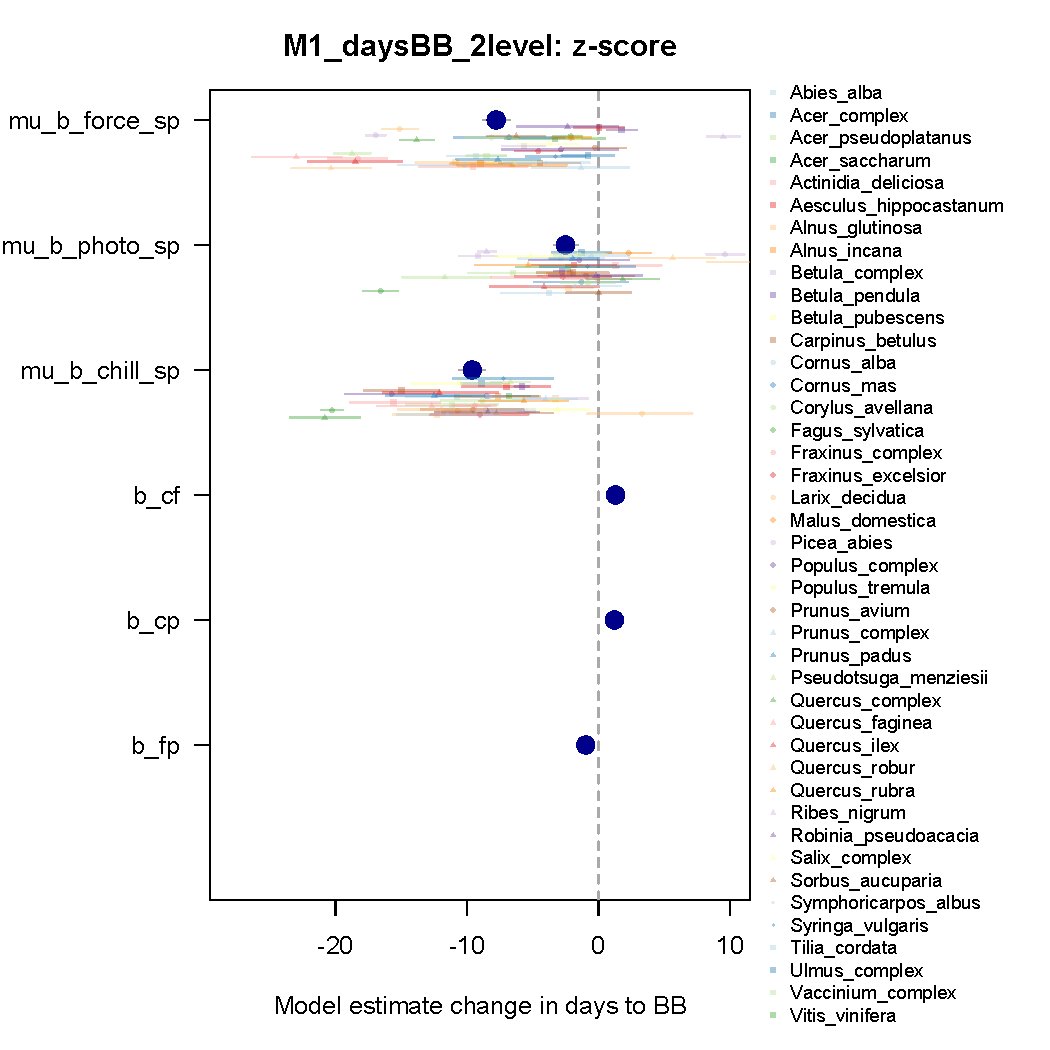
\includegraphics[width=1\textwidth]{..//..//analyses/bb_analysis/figures/M1winterZ_params_wcolor.pdf}
\caption{Z-score estimates using current model.}
  \label{fig:zscore}
\end{figure}
\clearpage


\begin{figure}[t!]
\centering
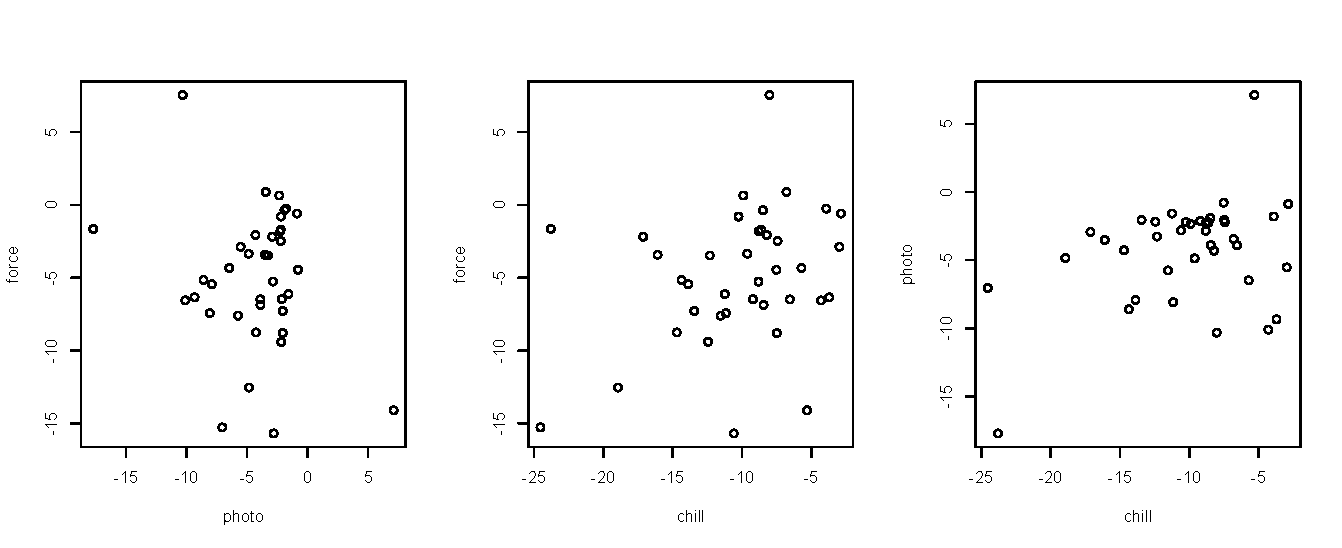
\includegraphics[width=1\textwidth]{..//..//analyses/bb_analysis/figures/M1winterZ_params_compspp.pdf}
\caption{Z-score estimates using current model compared across species.}
  \label{fig:sppcomp}
\end{figure}
\clearpage

\begin{figure}[t!]
\centering
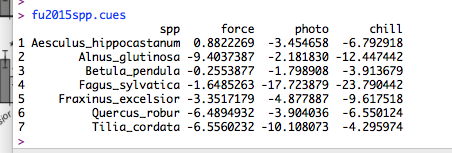
\includegraphics[width=0.8\textwidth]{figures/fuspp.png}
\caption{Lizzie's screen grab of the cues we estimate in the Fu et al. 2015 species}
  \label{fig:fuspp}
\end{figure}
\clearpage


\end{document}



%=======================================================================
% to-do listing
%=======================================================================



